\chapter{The 5C's of robotics}

\label{ch:introduction} 
\section{50 years of }
Most engineering problems are still solved as particular and stand-alone problems, so if a solution is not already available for that problem, a new one is developed with no concerns of making that solution re-usable for similar problems. Industrial research often force the researchers to opt for a quick, simple and cost-effective solution, ignoring the fact that tens or hundreds (maybe thousands!) of other engineers already addressed that problem, re-implementing the solution almost each time. Certainly it would be useful to reuse the same solution if possible, eventually improving it if it does not exactly fit the problem.
\section{Separation of concerns}
The separation of concerns if an approach to the code re usability problem promoted by BRICS. Researchers had identified 4 possible concerns, or behavior, that should be kept distinct with the goal of decoupling them and allowing an easy and standardized practice to re-use them across different applications, but also to make it easy to re-implement or substitute them within the \emph{same} application. These behaviors are computation, communication, coordination and configuration\cite{brics}.
\begin{wrapfigure}{r}{0.25\textwidth} %this figure will be at the right
	\label{fig:fivec}
	\centering
	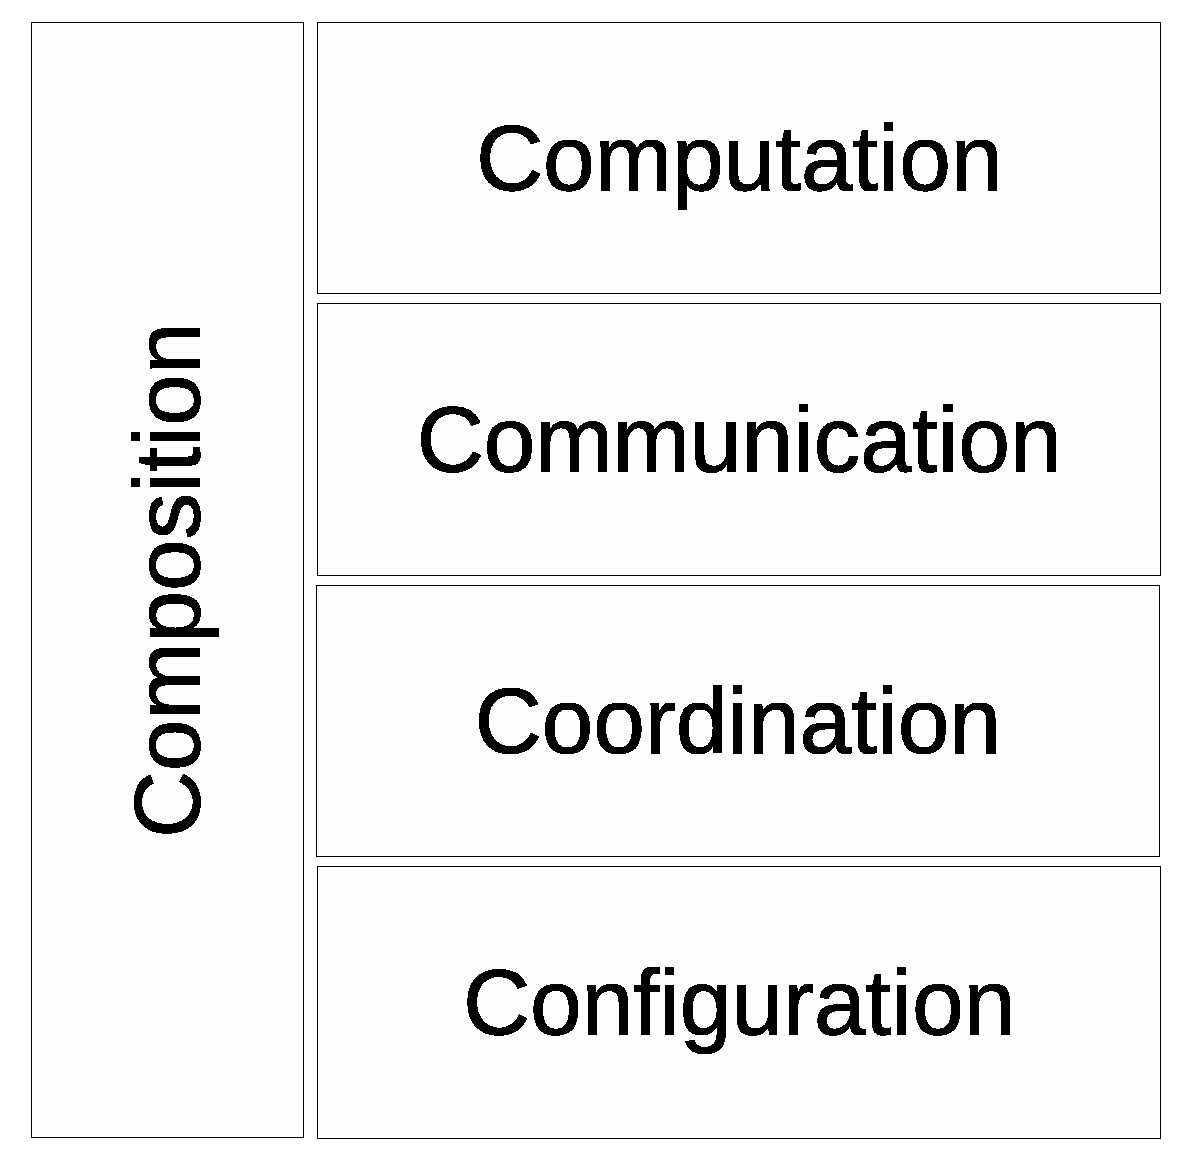
\includegraphics[width=0.5\textwidth]{5c}
%	The 4 behaviors of a system, glued by the composability property.
%		\label{fig:5c}
%		\ref{fig:5c}
\end{wrapfigure}
An additional concern was added to give this practice a good trade-off between scalability and complexity: more components can be composed to obtain a new component also having only one of the listed possible behaviors.
\subsection{Computation}
Computation is the core of a system functionality: it usually require read and/or write access to data, configuration and synchronization to produce the expected result.
\subsection{Communication}
Communication is responsible for data transmission between different computational components with the proper quality of service. A communication component usually store and retrieve data for computational components. In case a communication block do actually communicate with \emph{other} agents, it is named a \emph{bridge}.
\subsection{Coordination}
Coordination is responsible for the actual discrete behavior of the system and can be represented by a finite state machine, in other words it ensures the correct computational behavior at the correct time.
\subsection{Configuration}
Configuration is also responsible for the behavior of single computation or communication components; should be kept distinct and, indeed, configurable. Bad practice in software engineering is to hard-code configuration values; yet there are obvious exceptions like mathematical constants, e.g. $\pi$.
\subsection{Composition}
While separation of the previous 4 concerns gives a way to de-couple a system components, it is still necessary to introduce a trade-off between modularity and simplicity of the implementation. For this reason the last introduced behavior is \emph{composition} which gives the capability of combining components (with different concerns) into a macro component which in turn has one of the described behavior.




